\documentclass{article}
\usepackage{geometry,color,graphicx}
\usepackage{caption}
\usepackage{subcaption}
\usepackage{float}

\graphicspath{ {../plots/} }

\begin{document}

\title{Project 2: Monte Carlo methods for physical computations}

\author{Gabriel Smadi\\
  College of Engineering, \\
  College of Arts & Sciences, \\
  Physics Department, \\
  Syracuse University,\\
  \texttt{gsmadi@syr.edu}}
\maketitle

\begin{abstract}
  Monte Carlo methods are investigated for physical computations. Their usage is inspected by approximating the volume of a hypersphere. Also,
  using a Marcov Chain Monte Carlo (MCMC) algorithm, specifically the Metropolis algorithm, a ferromagnetic material is modeled by means of the Ising model.
\end{abstract}

\section{Introduction}
Monte Carlo methods can arrive at the same result of any deterministic solution through the means of randomness. Through the generation of random numbers, Monte
Carlo methods can achieve accurate results for several types of computations such as integrations and optimizations. However, Monte Carlo methods also prove useful
for simulating complex systems such as the Ising model, which is explored in the final section of this writing.

There are several aspects that make Monte Carlo methods attractive in a wide myriad of problems. First, using such methods it is relatively easy to incorporate
complex boundry conditions, such as the integration over a intricate surface. Also, these random methods can achieve better performance over higher dimensions than
other algoritmhs. For example, integration over $\ d$ dimensions, Simpson's Rule converges to the result with an error $\propto N^{-4/d}$, whereas Monte Carlo
integration converges to the result with an error $\propto 1/\sqrt N}$.

\section{Computation of a hypershere volume}

A enlightening Monte Carlo method problem is the computation of a hypersphere's volume. The simplest hypersphere to start with is one with 2 dimensions, most
commonly known as a circle.

Since a circle does not have sufficient dimensions to contain a volume, the analogue of volume for two dimension is area. Thus, for a circle, the area is given
by,

\begin{equation} \label{eq:circle_area}
  A_{circle} = \pi r^2
\end{equation}

To simplyfy matters, we compute the area of a circle of radius $\ r = 1$. The methodology employed to compute the area of a circle is described below,

\begin{enumerate}
  \item Generate a random coordinate $\ (x_{i}, y_{i}) $ inside a square of size 1 x 1.
  \item For a circle, the randomly generated point is inside the cricle if$\ x_{i}^2 + y_{i}^2 \leq r^2$.
  \item If randomly generated coordinate satisfies the condition in step 2, increment$\ n $ by 1.
  \item Perform step 1, 2, 3 for$\ N $ times.
\end{enumerate}

After completing the$\ N $ iterations, the total number of generated coordinates is contained in$\ n$. Thus, to approximate the area of the circle we
use the following expression,

\begin{equation} \label{eq:approx_circle_area}
  A_{circle} \approx 4(\frac{n}{N})r^2
\end{equation}

Equation \ref{eq:approx_circle_area} contains a factor of 4 because the generated coordinates lie inside a quarter of a circle. The ratio$\ n/N$ signifies
the number of points that fell inside the quarter circle versus the total number of points generated. Since we are computing the area of a circle of radius
$\ r = 1$, then by equation \ref{eq:circle_area} we should expect the area to be$\ \approx \pi$. In Figure \ref{fig:circle}, the simulation to approximate
the area of a circle is illustrated for different iterations.

\begin{figure}[H]
    \centering
    \begin{subfigure}[b]{0.30\textwidth}
        \scalebox{.4}{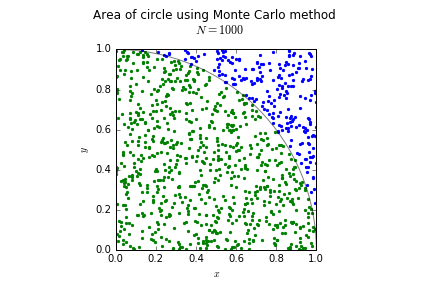
\includegraphics{circle_1000}}
        \label{fig:circle_1000}
    \end{subfigure}
    \begin{subfigure}[b]{0.30\textwidth}
        \scalebox{.4}{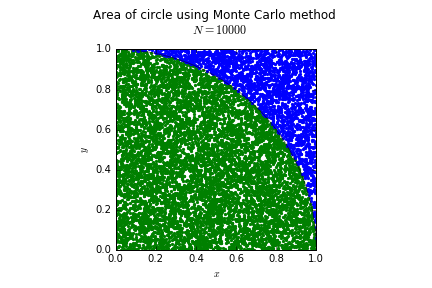
\includegraphics{circle_10000}}
        \label{fig:circle_10000}
    \end{subfigure}
    \begin{subfigure}[b]{0.30\textwidth}
        \scalebox{.4}{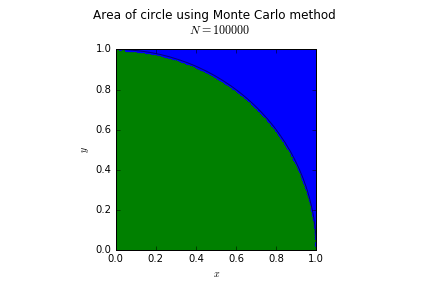
\includegraphics{circle_100000}}
        \label{fig:circle_100000}
    \end{subfigure}
    \caption{Approximation of of circle area via Monter Carlo method}\label{fig:circle}
\end{figure}

The simulation was carried out for $\ N = 10$ until $\ N = 100000000$. In the table below are the results, for several iterations.

\begin{table}[H]
  \begin{center}
    \begin{tabular}{|c|c|c|c|}
      \hline
      Iterations & Computed & Error \\
      \hline
      10 & 2.4 & 23.6\% \\
      \hline
      100 & 2.88 & 8.3\% \\
      \hline
      1000 & 3.132 & 0.3\% \\
      \hline
      10000 & 3.1316 & 0.3\% \\
      \hline
      100000 & 3.13648 & 0.2\% \\
      \hline
      1000000 & 3.139876 & 0.05\% \\
      \hline
      10000000 & 3.141691 & 0.003\% \\
      \hline
      100000000 & 3.141530 & 0.001\% \\
      \hline
    \end{tabular}
  \end{center}
  \caption {Circle area approximation for several  $N$ iteration.}
  \label{tab:circle_results}
\end{table}

The results from table \ref{tab:circle_results} can be appreciated visually in the figure below.

\begin{figure}[H]
  \begin{center}
    \scalebox{.8}{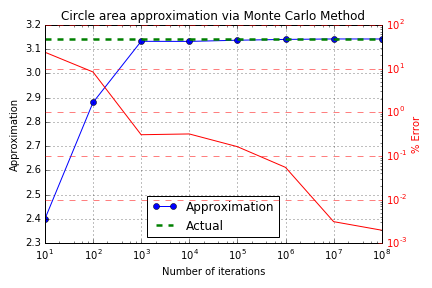
\includegraphics{dim_2_plot}}
  \end{center}
  \caption{Convergence of circle area approximation to actual value as $N\to \infty$}
  \label{fig:dim_2_plot}
\end{figure}

After $N = 1000$ the approximationn contains a \% Error of about 0.3\% or $A_{approx} \approx 3.132$,
which is quite close to the value of $\pi$.

Now, since we have seen satisfactory results for the approximation of the area of a circle we can do the same
with the volume of a sphere, where dimension $d = 3$. For a sphere, the procedure is the same as a circle the only different is that for
step 2, the condition is restated with an extra dimension as$\ x_{i}^2 + y_{i}^2 + z_{i}^2 \leq r^2$.

The volume of a sphere is given by,

\begin{equation} \label{eq:sphere_volume}
  V_{sphere} = \frac{4}{3}\pi r^3
\end{equation}

thus, for a sphere of radius $r = 1$, we should expect $ V_{sphere} \approx 4.189$. The convinience of using Monte Carlo methods for such
computations is that no matter the dimensionality of the computation, the form of equation \ref{eq:approx_circle_area} still holds even for a sphere of
dimension $ d = 3$. In other words, the form of equation \ref{eq:approx_circle_area} holds for any $d$. Hence, the task at hand, is to simply generate random
coordinates inside a hypercube (e.g. $d = 2$: square, $d = 3:cube$, etc.), count the ocurrences inside the hypersphere and compute the volume using
equation \ref{eq:approx_circle_area}.

Therefore, to generally define the approximation of a hypersphere for any dimension $d = 3$, in layman terms a sphere.

\begin{equation} \label{eq:hypersphere_volume}
  V_{hypersphere, d} = (\frac{n}{N})(2r)^d
\end{equation}

The factor of 2 is inside the exponent term becuase, for a circle we computed a quarter of the area, for a sphere we shall computed an eighth of the volume, and
so forth.

Below the simulation for computing the volume of a hypersphere of dimension $d = 3$ or in layman terms a sphere.

\begin{figure}[H]
\centering
    \begin{subfigure}[b]{0.30\textwidth}
        \scalebox{.4}{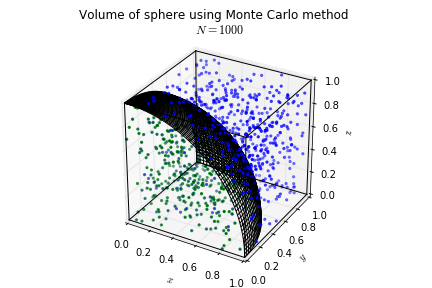
\includegraphics{sphere_1000}}
        \label{fig:sphere_1000}
    \end{subfigure}
    \begin{subfigure}[b]{0.30\textwidth}
        \scalebox{.4}{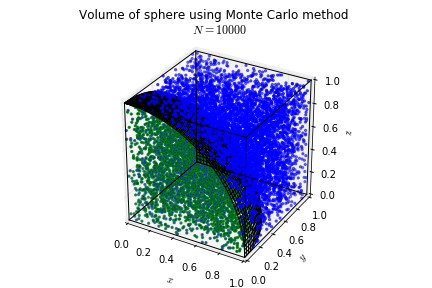
\includegraphics{sphere_10000}}
        \label{fig:sphere_10000}
    \end{subfigure}
    \begin{subfigure}[b]{0.30\textwidth}
        \scalebox{.4}{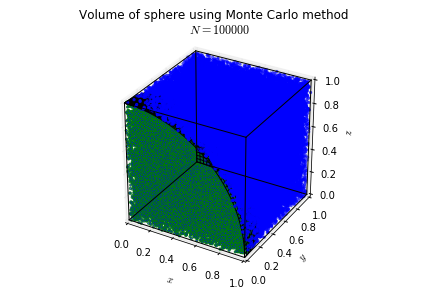
\includegraphics{sphere_100000}}
        \label{fig:sphere_100000}
    \end{subfigure}
    \caption{Approximation of sphere volume via Monter Carlo method}\label{fig:sphere}
\end{figure}

\begin{table}[H]
  \begin{center}
    \begin{tabular}{|c|c|c|c|}
      \hline
      Iterations & Computed & Error \\
      \hline
      10 & 4.8 & 14.6\% \\
      \hline
      100 & 4.64 & 10.8\% \\
      \hline
      1000 & 4.088 & 2.4\% \\
      \hline
      10000 & 4.1616 & 0.6\% \\
      \hline
      100000 & 4.1704 & 0.4\% \\
      \hline
      1000000 & 4.1858 & 0.07\% \\
      \hline
      10000000 & 4.188134 & 0.02\% \\
      \hline
      100000000 & 4.189403 & 0.01\% \\
      \hline
    \end{tabular}
  \end{center}
  \caption {Sphere volume approximation for several $N$ iteration.}
  \label{tab:circle_results}
\end{table}

\begin{figure}[H]
  \begin{center}
    \scalebox{.8}{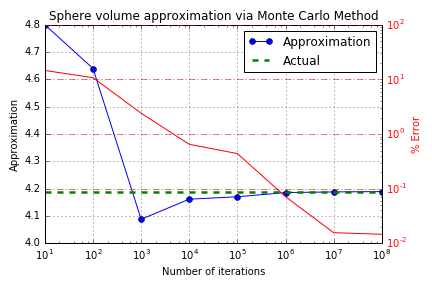
\includegraphics{dim_3_plot}}
  \end{center}
  \caption{Convergence of sphere volume approximation to actual value as $N\to \infty$}
  \label{fig:derivative}
\end{figure}

After $N = 10000$ the volume approximation is very close to the actual value, with a \% Error of 0.6\%.


Now that we have tested our Monte Carlo method for managable hypersphere configurations with satisfactory results, let us investigate
a higher dimensional hypersphere. From theory, the volume of a 10 dimensional hypersphere is given by,

\begin{equation} \label{eq:ten_dim_volume}
  V_{10-dim} = \frac{\pi^5}{120} r^{10}
\end{equation}

Hence, for a hypersphere of radius $r = 1$, $ V_{10-dim} \approx 2.55$.For 10 dimensions, the condition for checking if a
random coordinate is inside the hypersphere is given by,

\begin{equation} \label{eq:ten_dim_cond}
    \sum_{n=1}^{10}x_{i} \leq r^2
\end{equation}

where $x_{1} = x$, $x_{2} = y$, $x_{3} = z$, would be the typical x, y, z coordinate space we live in. Given the "curse of dimentionality",
visualizing the simulation would be cumbersome and unintuitive due to the difficulty of representing 10 dimentions. Thus, we view the results
directly in this case.

\begin{table}[H]
  \begin{center}
    \begin{tabular}{|c|c|c|c|}
      \hline
      Iterations & Computed & Error \\
      \hline
      10 & 0.0 & 100\% \\
      \hline
      100 & 0.0 & 100\% \\
      \hline
      1000 & 1.024 & 59.8\% \\
      \hline
      10000 & 2.8672 & 12.4\% \\
      \hline
      100000 & 2.580480 & 1.2\% \\
      \hline
      1000000 & 2.56 & 0.4\% \\
      \hline
      10000000 & 2.560205 & 0.4\% \\
      \hline
      100000000 & 2.542408 & 0.3\% \\
      \hline
    \end{tabular}
  \end{center}
  \caption {Volume approximation of 10 dimensional hypersphere for several  $N$ iteration.}
  \label{tab:circle_results}
\end{table}

\begin{figure}[H]
\centering
  \begin{center}
    \scalebox{.8}{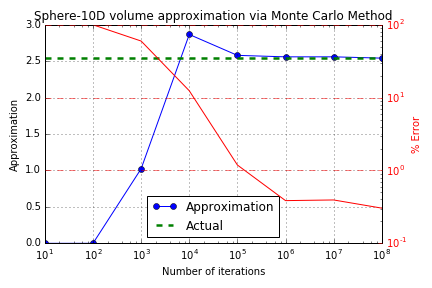
\includegraphics{dim_10_plot}}
  \end{center}
  \caption{Convergence of 10 dimensional hypersphere volume approximation to actual value as $N\to \infty$}
  \label{fig:derivative}
\end{figure}

For a 10 dimensional hypersphere, the approximate value converges closely to the actual value around $N = 10^{5}$.
Contrasting the results with the circle ($d = 2$) and sphere ($d = 3$), the general trend appears to be the more
dimensions, the larger the required N to converge to the actual value. Intuitively this would makes sense since
as the number of dimension $d$ is growing the less probable it is for a randomly generated coordinate to be inside
the hypersphere.


\section{Ising Model}

The Ising model is a model of ferromagnetism where phase transitions can be identified. The simplest and most approchable
configuration is a the Square-lattice Ising model and the one we shall be investigating. The model is laid out in a square
lattice of size $N = L \times L$. From this model we may study a set up observables, particularly, we shall be being attention
to the magnetization of the configuration.

The Hamiltonian of a particular location on the lattice is given by,

\begin{equation} \label{eq:hamilltonian}
  H_{i} = -J\sum_{j_{nn}} s_{i}s_{j}
\end{equation}

where, J is a coupling constant, $s_{i}$ is the location choosen to measure the energy and $s_{j}$ are the neighboring spins to $s_{i}$. In
simulation we shall take $J = +1$, which implies the material in question would be ferromagnetic. Also, in the implementation presented $k_{B}$ is
taken to be 1. Also, the ferromagnetic is absent of a magnetic field in our simulation.

The magnetization of the system is given by,

\begin{equation} \label{eq:total_spins}
  \langle{M}\rangle = \frac{1}{NN_{mc}}\sum_{s_{i},s{j}}^{N} s_{i, j}
\end{equation}

where $N$ is the size of the lattice, $N_{mc}$ is the number of monte carlo loops. The equation above will simply sum over all the spins in
the lattice and that will be the average magnetization. Note in theory, the average magnetization must be multiplied with a corresponding
probability, however, in this case the system is being updated by a corresponding probability thus such multiplication is not neccesary.

The important computational detail that concerns the Ising model implementation is deciding when and how to update the system.
This is where the Metropolis algorithm plays its part. The Metropolis algorithm is a Markov Chain Monte Carlo (MCMC),
that permits random sampling of a probability distribution. In our context, the probability distibution in concern is the
probability density of the systems energy, where the transition probability is given by $ e^{\delta H / k_{B}T}$. The Markov chain portion
of the algorithm is concerned with the random walk that will permit us to visit each state of the model that minimizes the change in energy
at a particular temperature. While, the Monte Carlo portion of the algorithm permits us to sample the system many times to obtain
an average value for an observable (e.g. magnetization, energy, etc.) at a particular state of the system. The diagram below shows the Metropolis
algorithm with is corresponding parts dissected.

\begin{figure}[H]
  \begin{center}
    \scalebox{.6}{\includegraphics{metropolis}}
  \end{center}
  \caption{Metropolis algorithm adapted from Kotze[4]}
  \label{fig:metropolis}
\end{figure}

For the simulation of the Ising model, the observables studied were $\langle{M^2}\rangle$ and $\langle{\left|M\right|}\rangle$. We also In the
implementation the Metropolis algorithm is used to update the Ising model for temperatures from 0.1 to 5.0 with 0.1 increments. Below we visualize
the simulation of 128 x 128 lattice Ising model for different temperatures.

\begin{figure}[H]
  \begin{center}
    \scalebox{.6}{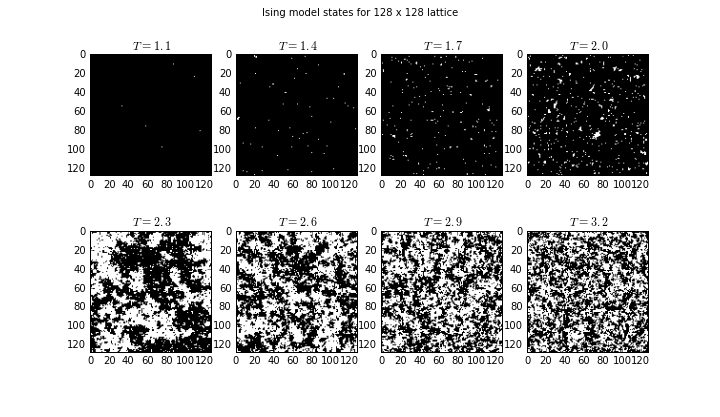
\includegraphics{ising_states}}
  \end{center}
  \caption{Evolution of ising model at different temperatures}
  \label{fig:ising_states}
\end{figure}

From the figure above we see how the spins are organized in parallel for low temperatures. As the temperature increase the spins start desorganizing themselves
randomly. Specifically, after the Curie temperature $T_{c}$ is where the spins start to get disorganize. Later, we shall find the Curie temperature by visualizing
magnetic susceptability.

The average magnetization for different lattice sizes can be appraciated in the figure below. Around the Curie temperature the spins are aligned completely either spin up or spin down. After
the Curie temperature, the spins average out the magnetization to zero.

\begin{figure}[H]
  \begin{center}
    \scalebox{.8}{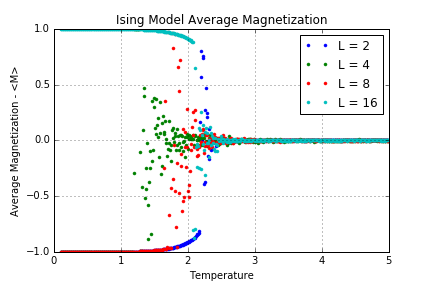
\includegraphics{avg_mag}}
  \end{center}
  \caption{Average magnetization for different lattice sizes}
  \label{fig:avg_mag}
\end{figure}

\begin{figure}[H]
  \begin{center}
    \scalebox{.8}{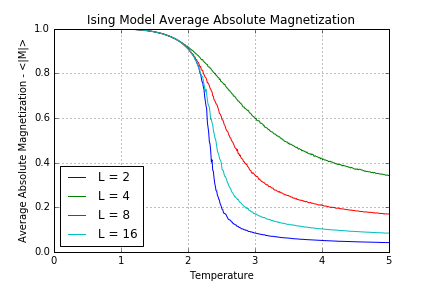
\includegraphics{avg_abs_mag}}
  \end{center}
  \caption{Absolute average magnetization for different lattice sizes}
  \label{fig:derivative}
\end{figure}

\begin{figure}[H]
  \begin{center}
    \scalebox{.8}{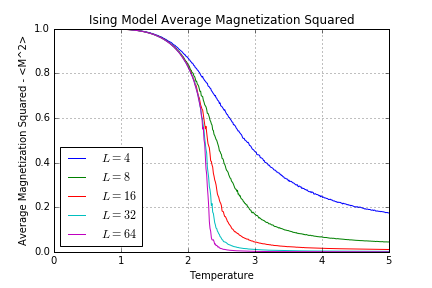
\includegraphics{avg_mag_squared}}
  \end{center}
  \caption{Normalized average magnetization squared for different lattices sizes}
  \label{fig:derivative}
\end{figure}


In the infinite volume limit, the magnetic susceptability converges at the Curie temperature $T_{c}$. In theory, the value of
the Curie temperature is given by,

\begin{equation} \label{eq:curie_temp}
  T_{c} = \frac{2}{\ln(1 + \sqrt{2})} =  2.269185
\end{equation}

To find our Curie temperature we must find the temperature where the magnetic susceptability is maximum. The largest lattice
size for which data was obtained is $N = 64 \times 64$. Thus we prefer this lattice for later computations. The magnetic susceptability was calculated as,

\begin{equation} \label{eq:mag_susc}
  \chi^{\prime}(T) = \frac{\langle{M^2}\rangle - \langle{M_{abs, avg}^2}\rangle}{k_{B}T}
\end{equation}

with uncertainty,

\begin{equation} \label{eq:mag_susc_uncert}
  \delta(\chi^{\prime}) = \delta(\langle{M^2}\rangle) + \delta(\langle{M_{abs, avg}^2}\rangle)
\end{equation}

The average absolute magnetization squared was used as suggested by Kotze given that using the average magnetization provided skewness
to the left for small lattice sizes. The figure below shows the magnetic susceptability obtained for several lattice sizes.

\begin{figure}[H]
  \begin{center}
    \scalebox{.8}{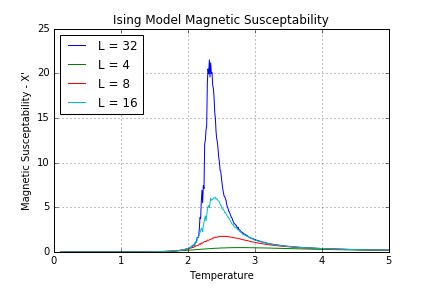
\includegraphics{mag_susc}}
  \end{center}
  \caption{Convergence of errors as $h\to 0$}
  \label{fig:mag_susc}
\end{figure}

From the data for a $64 \times 64$ we find the Curie temperature $T_{c}$, where,

\begin{equation} \label{eq:mag_susc_uncert}
  \chi_{max}^{\prime} = 64.59
\end{equation}

The temperature in terms of the magnetic susceptability is given by,


\begin{equation} \label{eq:chi_max}
  T(\chi^{\prime}) = \frac{\langle{M^2}\rangle - \langle{M_{abs, avg}^2}\rangle}{k_{B}\chi^{\prime}}
\end{equation}

which implies that,

\begin{equation} \label{eq:tc_approx}
  T_{c, approx} = T(\chi_{max}^{\prime}) = \frac{\langle{M^2}\rangle - \langle{M_{abs, avg}^2}\rangle}{k_{B}\chi_{max}^{\prime}}
\end{equation}

with uncertainty,

\begin{equation} \label{eq:tc_uncert}
  \delta T = \left|\frac{dT(\chi^{\prime})}{d\chi^{\prime}}\right|\delta\chi^{\prime} = \left|{\frac{\langle{M^2}\rangle - \langle{M_{abs, avg}^2}\rangle}{\chi^{\prime}^{2}}\right|(\delta\langle{M^2}\rangle + \delta\langle{M_{abs, avg}^2}\rangle)
\end{equation}

Thus, from equation \ref{eq:tc_approx}, we find that,

\begin{equation} \label{eq:tc_approx_val}
  T_{c, approx} = T(\chi_{max}^{\prime} = 64.59) = 2.31
\end{equation}

and with uncertainty,

\begin{equation} \label{eq:tc_uncert}
  \delta T = \frac{2.31}{64.59}(0.47 + 0.38) = 0.03
\end{equation}

Therefore, our final reportable value for $T_{c}$ is,

\begin{equation} \label{eq:tc_approx_val}
  T_{c} = 2.31 \pm 0.03
\end{equation}

\section{Conclusion}

We have seen the power of Monte Carlo methods for physical computations. From the calculations of the hypersphere volume we saw
how easy it is to incroporate boundry condition and to generalize these to greater dimensions. Also, we saw how quick these algorithms
can converge to actual values even for high dimensions as the 10 dimentional hypersphere.

Beyond te power for computations, Monte Carlo methods are ideal for simulations as well. From the Metropolis algorithm we saw how Monte
Carlo methods together with Markov chains can form a robust combination for sampling probability distributions. Using the Metropolis algorithm,
we were able to update and visualize the Ising model and to find the Curie temperature obtaining consistant results from theory.


\begin{thebibliography}{9}

  \bibitem{lamport94}
    Wikipedia contributors. \emph{Monte Carlo method.} Wikipedia, The Free Encyclopedia. Wikipedia, The Free Encyclopedia, 28 Mar. 2017.

  \bibitem{lamport94}
    Wikipedia contributors. "Markov chain Monte Carlo." Wikipedia, The Free Encyclopedia. Wikipedia, The Free Encyclopedia, 21 Feb. 2017.

  \bibitem{lamport94}
    Wikipedia contributors. "Square-lattice Ising model." Wikipedia, The Free Encyclopedia. Wikipedia, The Free Encyclopedia, 26 Mar. 2016.

    \bibitem{lamport94}
  	  Jacques Kotze,
  	  \emph{Introduction to Monte Carlo methods for an Ising model of ferromagnetism}.
      \tt{arXiv:cond-mat.stat-mech/0803.0217}

\end{thebibliography}
\end{document}
